\section{Installation}
Die im folgenden erläuterten Installationsschritte
sind in der Datei \verb|README.md| in dem Repository
\url{https://github.com/thomasstxyz/fhb-mcce-tmcsp-cloudnative-monitoring}.
genauer beschrieben.

\subsection{Ausgangssituation und Vorraussetzungen}
Als Basis-Betriebssystem wird Ubuntu Linux Server
in Version 20.04 \cite{ubuntuServerWebsite} verwendet.
Worauf die Docker Engine \cite{dockerEngineWebsite} installiert ist.

Für den Betrieb von Elasticsearch als Container muss der
Parameter \verb|vm.max_map_count| mittels \verb|sysctl|
auf den Wert \verb|262144| gesetzt werden.

\begin{verbatim}
sudo sysctl -w vm.max_map_count=262144
echo "vm.max_map_count=262144"|sudo tee \
--append /etc/sysctl.conf
\end{verbatim}

Als Quelle der Container Images wird die Repository
\verb|docker.elastic.co| herangezogen.
Es werden die Images \verb|elasticsearch/elasticsearch:8.2.2|, sowie
\verb|kibana/kibana:8.2.2| verwendet.
Hier ist anzumerken, dass alle Komponenten in einem
Elastic Stack mit der selben Versionsnummer installiert werden
müssen.

Die im folgenden installierten Container sollen alle
im selben internen Docker-Netzwerk \verb|elastic| laufen.
Dieses wird mit dem Befehl
\verb|docker network create elastic| erstellt.


\subsection{Start der Container}
Nun wird die initiale Instanz von Elasticsearch gestartet,
welche einen Elasticsearch-Cluster erstellt, mit anfangs
noch einem Knoten.
Dafür wird das \verb|elasticsearch:8.2.2| Container Image
mit \verb|docker run| und einer zusätzlichen Umgebungsvariable
\verb|-e ES_JAVA_OPTS="-Xms1g -Xmx1g"|,
gestartet. Dies erhöht den Heapspeicher, der für die
Java Runtime zur Verfügung gestellt wird.
Wird dies nicht gemacht, führt dies zu Schwierigkeiten
beim Starten von mehreren Elasticsearch-Containern
auf ein und derselben Maschine.
Die Ports 9200 und 9300 werden zur Host-Maschine weitergereicht,
sodass der Container auf diesen Ports auf der Host-Maschine
erreichbar ist. An den \verb|docker run| Befehl wird
dazu \verb|-p 9200:9200 -p 9300:9300| hinzugefügt.
Mit \verb|--net elastic| wird der Container dem zuvor erstellten
Netzwerk zugeteilt, und mit \verb|--name es01| wird der Name
des Containers definiert.
Dies führt zu folgendem Befehl:

\begin{verbatim}
	docker run -d \
	-e ES_JAVA_OPTS="-Xms1g -Xmx1g" \
	--name es01 \
	--net elastic \
	-p 9200:9200 -p 9300:9300 \
	-it \
	docker.elastic.co/elasticsearch/elasticsearch:8.2.2
\end{verbatim}

Nach dem Absetzen des \verb|docker run|-Befehls werden
mehrere Informationen auf die Konsole ausgegeben. Diese sollten
kopiert und an einem sicheren Ort abgespeichert werden.
Dies sind:

\begin{itemize}
	\item Passwort des elastic user
	\item Kibana enrollment token
	\item Elasticsearch enrollment token
\end{itemize}

Sollte das Password einmal zurückgesetzt werden müssen,
kann dies der Befehl
\verb|bin/elasticsearch-reset-password| im Container durchführen.

Außderdem wird auf die Konsole der Befehl ausgegeben, der zum
hinzufügen weiterer Elasticsearch-Cluster-Knoten notwendig ist.
Wird dieser ebenfalls unter Docker betrieben, muss hierfür lediglich
der Enrollment Token als \verb|-e ENROLLMENT_TOKEN="<token>"|
Umgebungsvariable beim \verb|docker run|-Befehl angegeben werden.

Nun wird Kibana ebenfalls als Docker Container gestartet.
Der Port 5601 wird zur Host-Maschine durchgereicht,
auf diesem ist das Web Interface zu erreichen.
Dies führt zu folgendem Befehl:

\begin{verbatim}
docker run -d \
--name kib-01 \
--net elastic \
-p 5601:5601 \
docker.elastic.co/kibana/kibana:8.2.2
\end{verbatim}

Jetzt kann das Kibana Web Interface im Browser
unter \url{http://<instance_ip>:5601} geöffnet werden.
Zunächst wird der Benutzer aufgefordert das Enrollment Token
von Elasticsearch,
und einen Security Code einzugeben, welcher auf der Konsole ausgegeben wird.
Dann kann sich mit dem User \verb|elastic| und dem generierten Passwort eingeloggt werden.

\section{Weiterführendes Setup}
Erfolgreich im Web Interface angelangt, ist es zu empfehlen,
einen sogenannten Fleet Server aufzusetzen. Dieser ist für eine
einheitliche Verwaltung der Elastic Agents zuständig, also
die Systeme, die in Folge überwacht werden sollen.
Um den Fleet Server zu initialisieren, muss nur zu
\url{http://<instance_ip>:5601/app/fleet} navigiert,
und den Schritten gefolgt werden.

Schließlich können diverse sogenannte Integrationen \cite{elasticIntegrationsWebsite}
für Elasticsearch im Kibana Web Interface installiert werden.
Integrationen für open-source Software wie Apache httpd oder NGINX,
oder auch Integrationen in verschiedenste Cloud-Umgebungen und dessen
Systeme wie Amazon S3, GitLab, oder Atlassians Jira.

\section{Logs}
Im Reiter \verb|Observability>Logs>Stream| können alle zusammengeführten
Logs eingesehen und durchsucht werden (siehe Fig. \ref{fig:logsStream}).

\begin{figure}[h]
	\centering
	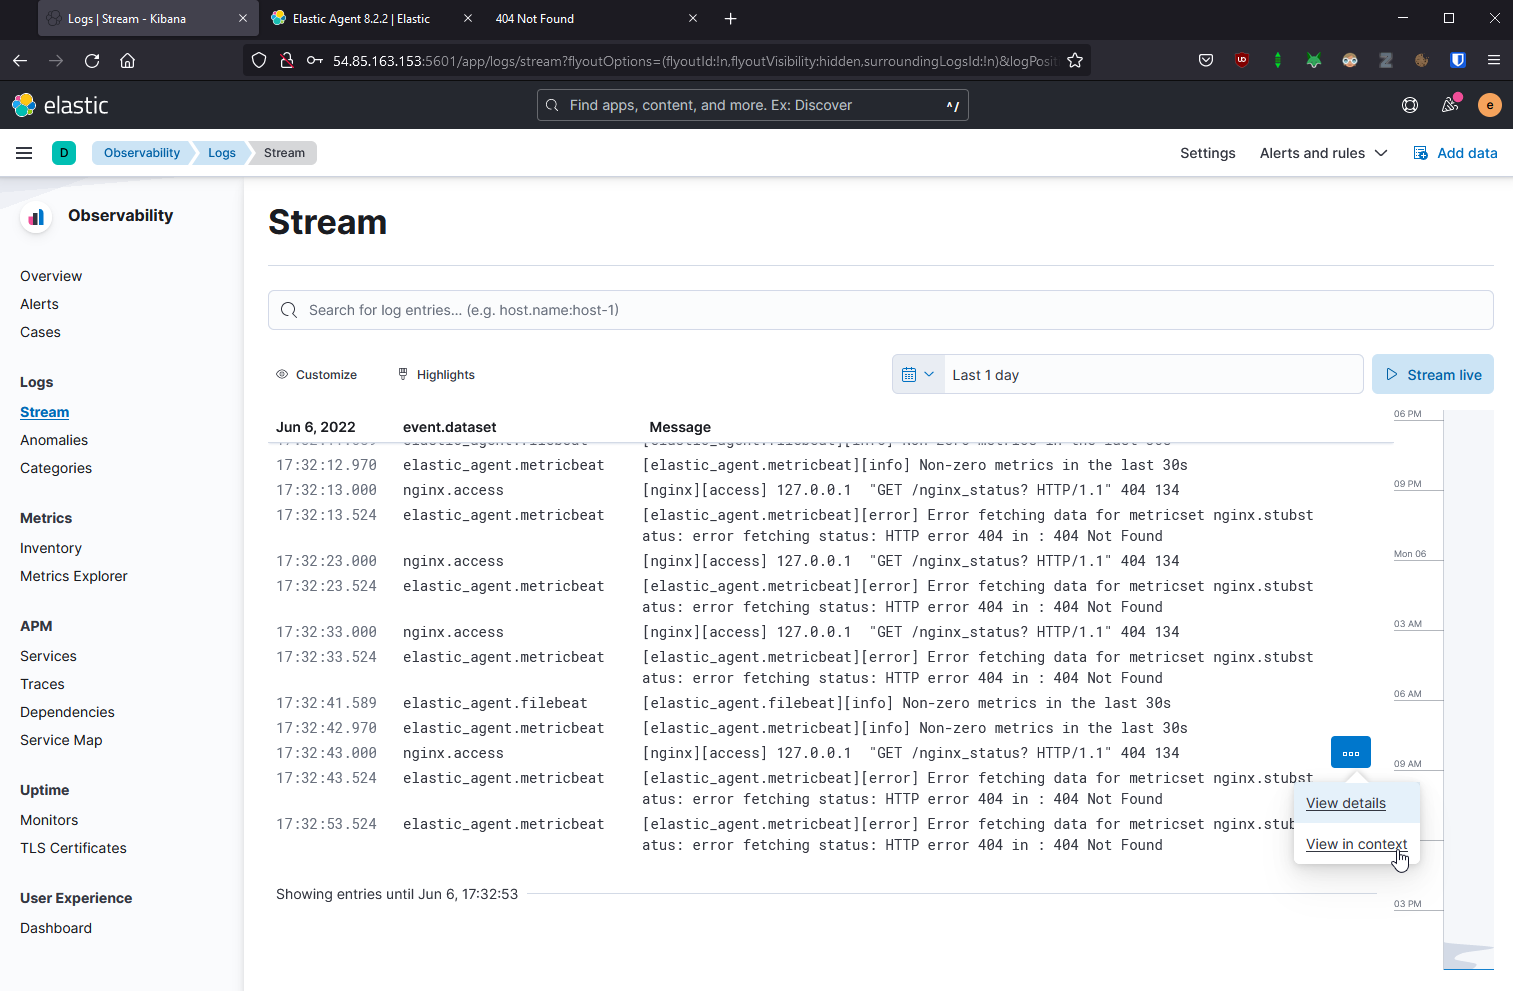
\includegraphics[width=.99\linewidth]{fig/logsStream.png}
	\caption{Zusammenführung aller Logs als Stream}
	\label{fig:logsStream}
\end{figure}

Nun kann beispielsweise die Ansicht auf die Nginx Logs eingeschränkt werden
(siehe Fig. \ref{fig:logsStreamNginx}).

\begin{figure}[h]
	\centering
	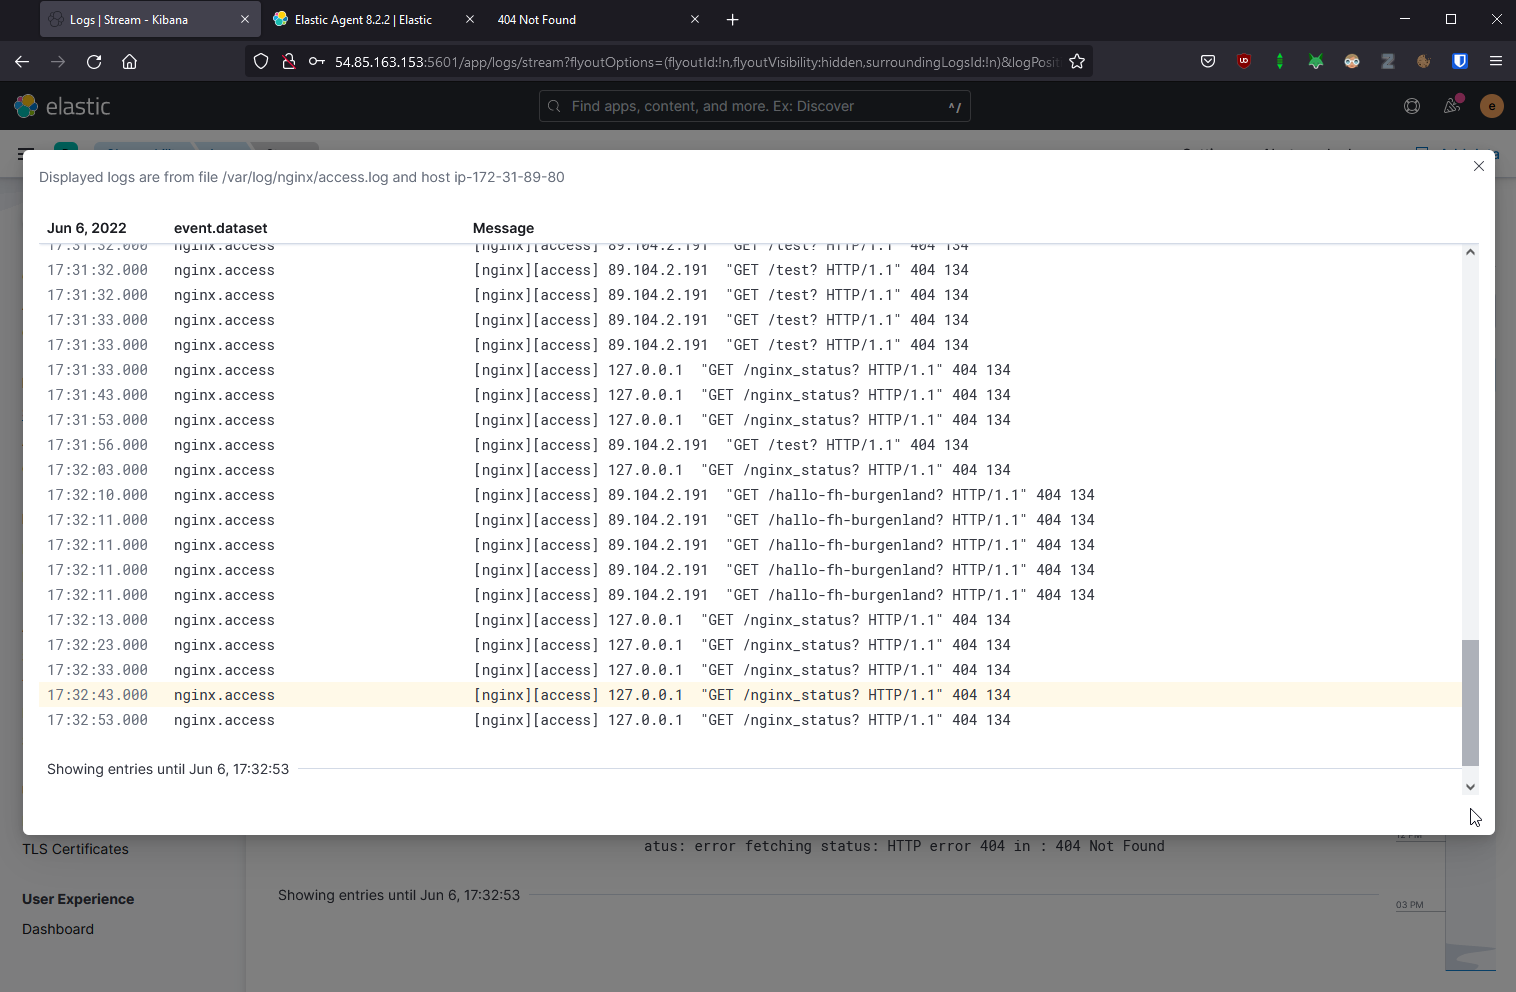
\includegraphics[width=.99\linewidth]{fig/logsStreamNginx.png}
	\caption{Nginx Logs}
	\label{fig:logsStreamNginx}
\end{figure}

\section{Analyse und Visualisierung}
In der \verb|Visualize Library| kann eine visuelle Darstellung
der Zugriffe auf Nginx angesehen werden (siehe Fig. \ref{fig:nginxAccessMap}),
bezüglich der Quell-IP-Addresse,
wird auf die Geolocation geschlossen. Somit können Besucher einer Website
geografisch geortet bzw. statistische Auswertungen durchgeführt werden.
Eine ähnliche Ansicht existiert auch als Heatmap.

\begin{figure}[h]
	\centering
	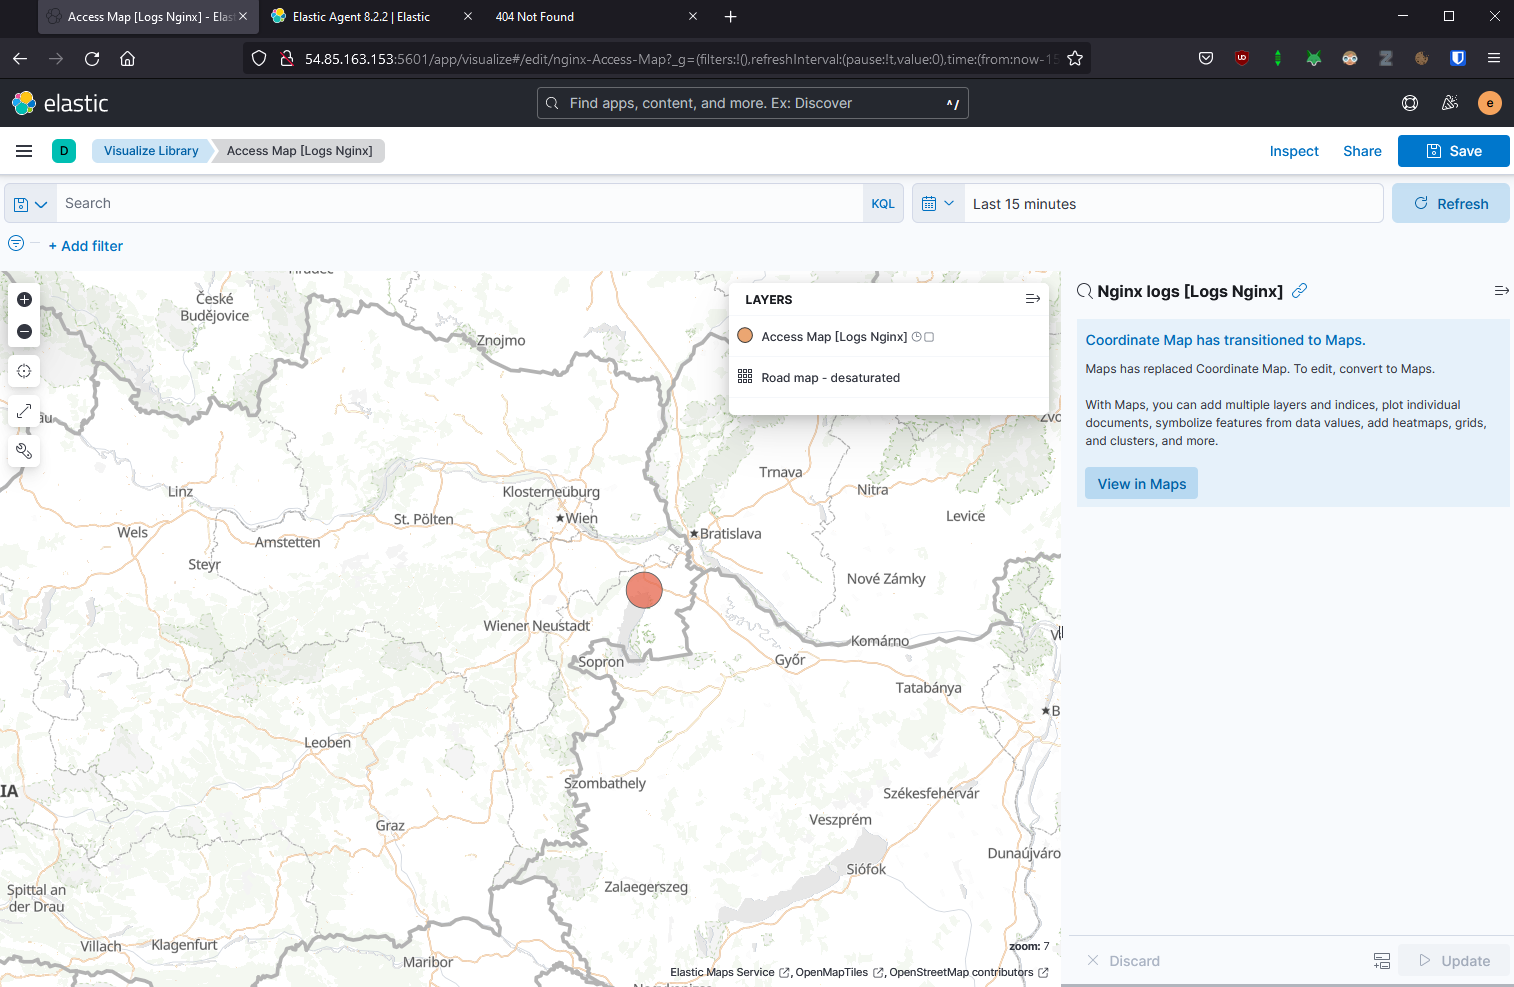
\includegraphics[width=.99\linewidth]{fig/nginxAccessMap.png}
	\caption{Nginx Access Map}
	\label{fig:nginxAccessMap}
\end{figure}

\section{Metriken}
Im Reiter \verb|Observability>Metrics>Inventory| können host-basierte
Metriken wie Prozessor-Auslastung, Arbeitsspeicherverbrauch,
Netzwerklast, und auch weitere Integrationen wie Metriken
welche auf Basis der Nginx Logs gebildet werden, angesehen werden
(siehe Fig. \ref{fig:metrics}).

\begin{figure}[h]
	\centering
	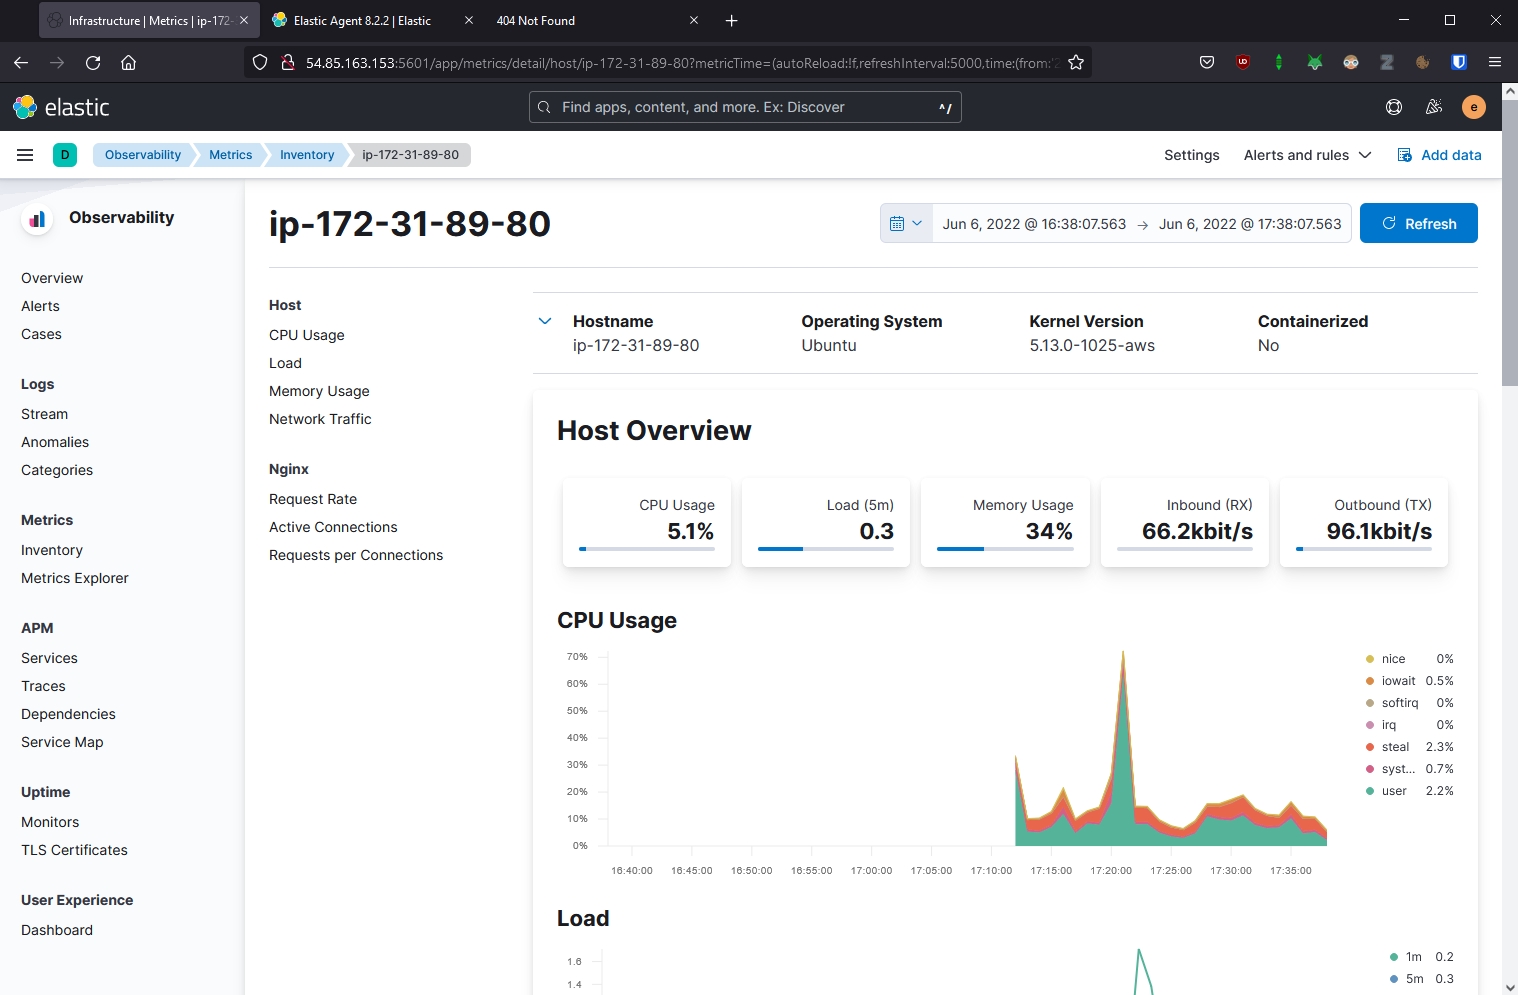
\includegraphics[width=.99\linewidth]{fig/metrics.png}
	\caption{Metriken}
	\label{fig:metrics}
\end{figure}
